\chapter{Simulating the Lyman-alpha forest} \label{chap:sherwood}
In Section \ref{chapter:intro} we discussed how the Lyman-$\alpha$ forest is sentive to multiple physical parameters, such as the low-gas temperatures, velocities, densities, etc. Each possible state of the IGM's ionized low-density gas can lead to different absorption spectra and different forms of the forest. Hydrogen reionisation finishes at $z<5.3$ \cite{Bosman_2022}. Hence, at low redshift, there is no neutral hydrogren to produce absoprtion features, and we have complete transmission of the Lyman-$\alpha$ flux withput features, which means we cannot extract information about the IGM through this process. On the other end, at high redshifts, $z>6$, the hydrogren is not sufficiently ionized and total absoprtion of quasar continuum by neutral hydrogen generates long Gunn-Peterson troughs.
Hence, the Lyman-$\alpha$ forest at $2<z<5$ is a powerful probe of the state of the IGM at scales and redshifts not accessible by any other observable \cite{Hernquist__1996}. As a consequence, simulations of the Lyman-$\alpha$ forest are typically carried out at said redshift range.














\section{The Sherwood simulation suite}\label{sec:sherwood suite}
Lyman-$\alpha$ simulations are typically based on cosmological simulation codes.
In this work, we will mainly focus on the \texttt{SHERWOOD} simulation suite\footnote{\url{https://www.nottingham.ac.uk/astronomy/sherwood/}} \cite{Bolton_2016}, which are based on the \texttt{GADGET-2} developped by Volker Springel \cite{Springel_2005}. \texttt{GADGET-2} uses the Lagrangian formulation of fluid dynamics to trace the evolution of fluid particles.


\texttt{GADGET-2} traces non-interacting dark matter (as described by the collisionless Boltzmann equation) by sampling phase space with a finite number of particles and solving their dynamics. The dynamics of such particles are subject to the Hamiltonian

\begin{equation}
        H=\sum_i\frac{\boldsymbol{p}_i^2}{2 m_i a(t)^2}+\frac12\sum_{ij}\frac{m_im_j \varphi(\boldsymbol{x}_i-\boldsymbol{x}_j)}{a(t)},
\end{equation}
where $\boldsymbol{x}$ are the comoving positions, $a$ the scale factor, $\boldsymbol{p}$ the canonical momenta and $m$ the particle masses.

On the other hand the gas particles are traced using Smoothed Particle hydrodynamics (SPH). SPH describes a fluid by means of a finite set of tracer particles that sample the local state of the fluid. Then, smooth quantities are obtained by using a smoothing kernel to interpolate between the tracer's properties. The equation of motion for the SPH particles is then
\begin{equation}
        \frac{\mathrm{d}\boldsymbol{v}_i}{\mathrm{d}t}=-\sum_{j=1}^Nm_j\left[f_i\frac{P_i}{\rho_i^2}\nabla_iW_{ij}(h_i)+f_j\frac{P_j}{\rho_j^2}\nabla_iW_{ij}(h_j)\right],
\end{equation}
with
\begin{equation}
        f_i=\left[1+\frac{h_i}{3\rho_i}\frac{\partial\rho_i}{\partial h_i}\right]^{-1}.
\end{equation}
Here, $W$ is the smoothing kernel, $h_i$ are smoothing lengths parameters, $P_i$ are the pressures associated with the particles and $\rho_i$ their densities. For more details see the original paper \cite{Springel_2005}.



Gravity is the driving force for strucuture formation in the Universe, but its long-range nature makes it challenging to implement efficiently. \texttt{GADGET-2} implements a gravitational algorithm that ensure sufficient spatical adaptability by using a hierarchical multipole expansion. By using a tree-like approach, we can compute the force applied to a particle in compelcity $\mathcal{O}(log(N))$ instead of $\mathcal{O}(N)$, where $N$ is the number of particles. The algorithm works by subdividing the space into octants, such that each leaf contains a single particle. The net force on a particle is then calculated by traversing the octree and replacing distant cell by a single body, thus reducing the number of needed terms. This process is also called the \emph{Barnes-Hut} algorithm, see Figure \ref{fig: 2D Barnes Hut} for an Illustration of it.

\begin{figure}
        \centering
        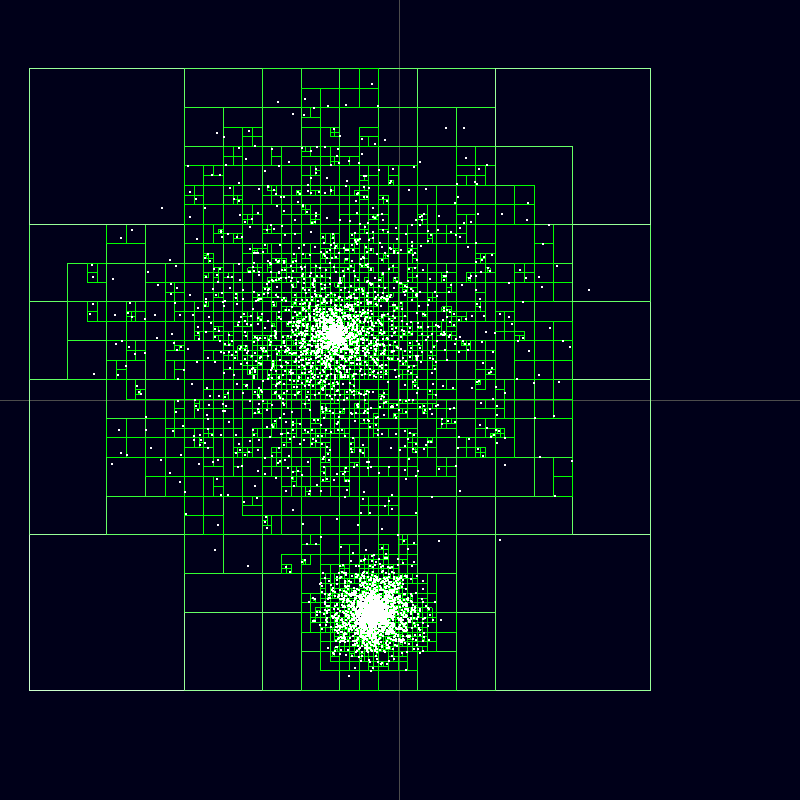
\includegraphics[width=0.5\textwidth]{img/ML/Barnes_hut_tree.png}
        \caption{An octree generated using the Barnes-Hut algorithm for a set of particles (in white) in a 2D space.}
        \label{fig: 2D Barnes Hut}     
\end{figure}

The  dynamics of the system are then governed by the interaction potential
\begin{equation}
        \nabla^2\varPhi(x)=4\pi G(\rho-\overline{\rho}).
\end{equation}

The \texttt{SHERWOOD} suite implements the effect of WDM by suppressing the initial power spectrum as described in \cite{Viel_2005}. In this approach, the effects of the warm dark matter free-streaming length on the matter distribution are described by a transfer function $T(k)$

\begin{equation}
        T(k)^2=\frac{P(k)_{\Lambda\mathrm{WDM}}}{P(k)_{\Lambda\mathrm{CDM}}},
\end{equation}
where $P(k)$ is the matter power spectrum (see Section \ref{sec:statistics sher} for more details). For pure thermal WDM models, as the ones we consider in this work, the transfer function can be approximated by:

\begin{equation}
        T(k)=[1+(\alpha k)^{2\nu}]^{-5/\nu},
\end{equation}
where $\nu\approx 1.12$ and $\alpha$ is related to the WDM particle mass by
\begin{equation}
        \alpha \propto \left( \frac{m_\mathrm{WDM}}{1 \mathrm{KeV}} \right)^{-1.11}.
\end{equation}
The initial coniditons are then generated at $z=99$ using the matter power spectrum, see \cite{Bolton_2016} for more details.

On top of the hydrodynamics and gravity, the Sherwood code implements a variety of relevant physical process that contribute to the state of the IGM and the Lyman-$\alpha$ forest. The simulations calculate the photo-ionisation and photo-heating for the gas (assumed to be in ionisation equilibrium) by using a uniform ionising UV backgorund as described in \cite{Haardt2012}. Instead of following the star formation process, dense and cold gas particles ($\Delta>1000$ and $T<10^5$K) are converted into collisionless particles. The runs discussed here do not include AGN feedback, which has a small effect on the Lyman-$\alpha$ forest at high redshift.

In our work, we use a subset of the \texttt{SHERWOOD} suite described in \cite{sherwood_wdm}. All boxes are of size 20h$^{-1}$cMpc, with $2\times 1024^3$ particles. The mass for gas and dark matter particles is, respectively, $5.37\times 10^5h^{-1}M_\odot$ and $9.97\times 10^4h^{-1}M_\odot$. In Table \ref{tab: Sherwood} we summarise the runs used in this work.


\begin{table}
        \caption[]{List of the \texttt{SHERWOOD} runs used in the work.
        All box sizes are 20h$^{-1}$. The table shows the mean temperature of the IGM $T_0$ at redshift $z=4.4$, the redshift of reionisation, and the set of WDM masses included. We work with the inverse WDM mass and consider 0 to correspond to the CDM reference run.}
           \label{tab: Sherwood}
       $$ 
           \begin{array}{p{0.3\linewidth}ccc}
              \hline
              \noalign{\smallskip}
              Run      &  T_0 {[\mathrm{K}]}\ (z=4.4) &z_\mathrm{rei}^\mathrm{end}& \mathrm{WDM} [\mathrm{KeV}^{-1}] \\ 
              \noalign{\smallskip}
              \hline
              \noalign{\smallskip}
              L20-ref & 10556 &6.00&\{0,\frac{1}{2}, \frac{1}{3}, \frac{1}{4}, \frac{1}{8}, \frac{1}{12} \}     \\
              L20-ref-hot           & 12161&6.01  &\texttt{"}\\
              L20-ref-cold     & 9862  &5.98&       \texttt{"}     \\
              \noalign{\smallskip}
              \hline
           \end{array}
       $$ 
     \end{table}
The reference run is L20-ref. We will refer to the dataset consisting on this run as \texttt{SHERWOOD} in what follows. We also use two runs with varied thermal parameters L20-ref-hot and L20-ref-cold. The dataset consisting on all 3 runs will be denoted as \texttt{SHERWOOD THERMAL} in this work.

We conclude this section by visually inspecting the \texttt{SHERWOOD} data, to give a broad intuition of how the IGM fields behave. In Figure \ref{fig: 2D density image} we show a 2D neutral hydrogren overdensity field generated using the \texttt{SHERWOOD} suite at $z=4.2$ for multiple WDM models. The simulation size is 20h$^{-1}$cMpc. On the horizontal axis, we linearly interpolate the density field for the WDM models to show the effect or multiple DM candidates on the density field.
\begin{figure}[ht]
        \centering
        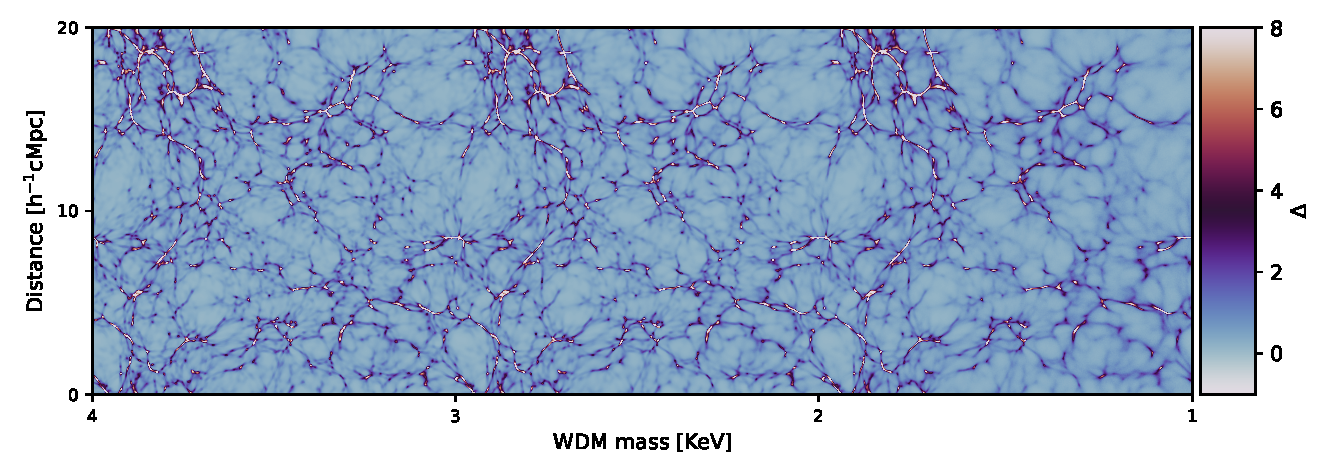
\includegraphics[width=0.99\textwidth]{img/ML/density_image_wdm.pdf}
        \caption{A 2D neutral hydrogren overdensity field generated using the \texttt{SHERWOOD} suite at $z=4.2$ for multiple WDM models. The simulation size is 20h$^{-1}$cMpc. On the horizontal axis, we linearly interpolate the density field for the WDM models to show the effect or multiple DM candidates on the density field.}
        \label{fig: 2D density image}     
\end{figure}
In Figure \ref{fig: 1D density skewer} we show a  1D neutral hydrogren overdensity field at $z=4.4$ along a 20h$^{-1}$cMpc Sherwood skewer for the CDM model run. Note how the density field is periodic, since the Sherwood simulations implement periodic boundary conditions. Most of the gas is close to the mean density $\Delta \sim 1$, with local overdensities that can generate $\Delta \sim 20$ corresponding to regions where there is a positive flow of gas.
\begin{figure}
        \centering
        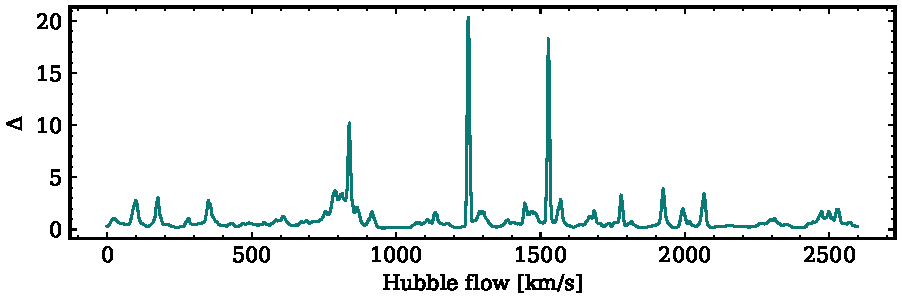
\includegraphics[width=0.99\textwidth]{img/ML/Skewer_density.pdf}
        \caption{A 1D neutral hydrogren overdensity field at $z=4.4$ along a 20h$^{-1}$cMpc Sherwood skewer for the CDM model run.}
        \label{fig: 1D density skewer}     
\end{figure}










\section{Obtaining mock Lyman-alpha skewers from cosmological simulations}
The \texttt{SHERWOOD} simulation suite described in Section \ref{sec:sherwood suite} generates as output the low-density IGM's overdensity, hydrogen neutral fraction, sightline velocity, temperature and the redshift of every pixel. For each run, recall that those fields form a $(5000,2048)$ array for all 5000 sightlines. From such data, we can use Equation \ref{eq:lyman opacity} to compute the simulated Lyman-$\alpha$ sightlines. We implement the code in Python and descritise the integral in Equation \ref{eq:lyman opacity} to sum over all 2048 pixel in the skewer. We use the values for the recombination coefficient in \cite{Luki__2014}.

In our code, we consider two different implementations for the Voigt profile, which is non-analitical. Firstly, we exploit the relationship with the Faddeeva function. The Faddeeva function is implemented in Scipy under \texttt{scipy.special.wofz} for optimized computation. Let us prove a relationship between the Faddeeva function and the Voigt function. Let $z=x+iy$.
The Faddeeva function $w(z)$ is defined as

\begin{equation}
    w(z)=\frac{i}{\pi} \int_{-\infty}^{\infty} \frac{e^{-t^2}}{z-t}dt
\end{equation}
and we have 
\begin{equation}\label{eq:FAD}
    Re \left( w(z=x+iy) \right)=V(x,y)
\end{equation}
The proof is trivial:
\begin{equation}
    \begin{split}
        Re\ i \int_{-\infty}^{\infty} \frac{e^{-t^2}}{z-t}dt
        &= Re\ i \int_{-\infty}^{\infty} \frac{e^{-t^2} (x-t-iy)}{(x-t)^2+y^2}dt\\
        &=y\int_{-\infty}^{\infty} \frac{e^{-t^2}}{(x-t)^2+y^2}dt
    \end{split}
\end{equation}

We consider a second implementation of the Voigt function by leveraging a power series expansion known as the Tepper-Garcia approximation \cite{Tepper_Garc_a_2006}. The Tepper-Garcia approximation is
\begin{equation}\label{eq:Tepper}
        V(x,y)\approx e^{-x^2}\left( 1-\frac{2y}{\sqrt{\pi}} K(x) \right),
\end{equation}
with
\begin{equation}
        K(x)=\frac1{2x^2}\left[(4x^2+3)\left(x^2+1\right)\mathrm{e}^{-x^2}-\frac1{x^2}(2x^2+3)\sinh x^2\right].
\end{equation}
As can be seen from the Tepper-Garcia approximation, the Voigt function is a modified Gaussian function. Figure \ref{fig: VOIGT APPROX} shows a comparison between the Faddeeva and Tepper-Garcia implementations of the Voigt function for multiple values of the $y$ parameter. Since in our problem typical recombination coefficients are of order $10^{-10}$cm$^3$s$^{-1}$, both implementations are essentially equivalent.

\begin{figure}[ht]
        \centering
        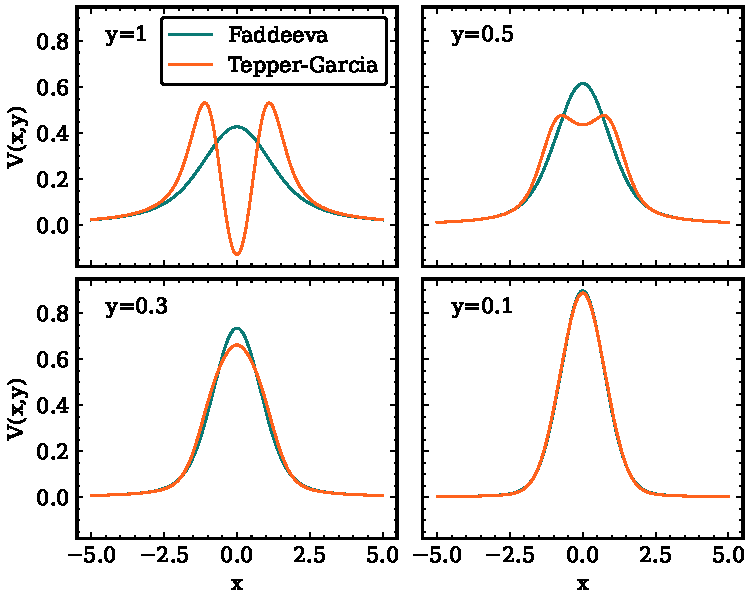
\includegraphics[width=0.8\textwidth]{img/ML/TP-FA.pdf}
        \caption{Comparison of the Voigt function $V(x,y)$ that is included in Equation \ref{eq:lyman opacity} implemented using the relation with the Faddeeva function in Equation \ref{eq:FAD} and the Tepper-Garcia approximation in Equation \ref{eq:Tepper}.}
        \label{fig: VOIGT APPROX}     
\end{figure}

An important aspect when simulating Lyman-$\alpha$ sightlines is boundary conditions. In fact, the simulation boxes in the \texttt{SHERWOOD} suite and other cosmological codes implement periodic boundary conditions. This means that a physical quantity $Q$ satisfies
\begin{eqnarray}
        Q(0)=Q(L),
\end{eqnarray}
where $L$ is the length of the simulation box. This condition also applies to the density field, temperature field, etc. Periodic boundary conditions allow implementing relevant physical conditions, such as conserved quantities, in the simulation volume. As a consequence, we would like the optical depth fields generated using the \texttt{SHERWOOD} data to also implement periodic boundary conditions. This will be the case if every pixel in the sightline has the approxmiate same environment has a translational by the skewer length. To achieve this in a computationally efficient manner, observe that in Equation \ref{eq:lyman opacity}, for $\alpha\to 0$, the amplitude of the Voight profile is set by $b(T)\sim 10$ km/s for $T\sim 10^4$. Since the pixel scale is $\sim 1$ km/s, the Voigt profiles only influence neaby pixels. As such, let us fix a pixel $i$ on which we wish to calculate the optical depth. Then, we iterate over all pixels $j$ and evaluate the condition $|z[i]-z[j]| < L/2$. If this condition is true, we use Equation \ref{eq:lyman opacity} to compute the contribution. If the condition is false, then we use the pixel at $z[j]\pm L/2$ that is closer to $z[i]$. This allows us to in include (approximately) periodic boundary conditions with a complexity $\mathcal{O}(N^2)$ where $N$ is the number of pixels. For reference, see the optical depth field in Figure \ref{fig: skewer sherwood}, where we have applied this procedure.



\section{Peculiar velocities and optical depth-weighted quantities}\label{sec: optical depth weighted}
Equation \ref{eq:lyman opacity} relates properties of the low-density hydrogen in the IGM to the Lyman-$\alpha$ flux field. Each density pixel contributes to the optical depth at any fixed pixel by a quantity proportinal to its density and to the absoprtion profile. However, note that the velocity contributes by shifting the center of the absoprtion profile. As a consequence, the small-scale peculiar velocities of the absorbers due to structure formation wash out the correlation between the overdensity $\Delta$ and $\tau$ fields. A second undesirable effect of the velocity is that it can create potential degeneracies between the gas properties and the flux. In fact, The effect of the velocity field can be captured by considering a shifted density field generating the same flux field. These two problems mean that it is not feasible to recover the real $\Delta$ from the flux. To better correlate the flux features with the density and temperature features and neglect the effects of peculiar velocities, it is common in the literature to work with optical depth-weighted quantities \cite{_oltinsk__2021}. Such quantites allow for a better identification of the gas associated with a certain absoption profile. Optical depth quantities are highly correlated to real quantities and act as a proxy for the latter \cite{Schaye1999}.

We define the optical depth-weighted overdensity field, $\Delta_\tau$, as
\begin{equation}\label{eq: OD weighted}
        \Delta_{\tau,i}=\sum_j \tau_{ij} \Delta_j /\tau_i,
\end{equation}
where $\tau_{ij}$ is the contribution to optical depth at pixel $i$ by pixel $j$. Equation \ref{eq: OD weighted} can also be used to compute the optical depth-weighted temperature. Figure \ref{fig: skewer sherwood} shows a 20h$^{-1}$cMpc \texttt{SHERWOOD} CDM skewer at $z=4.4$ with 2048 pixels. We show the hydrogen overdensity $\Delta$, temperature $T$ and velocity along the sightline $V$, Lyman-$\alpha$ optical depth and flux computed according to \ref{eq:lyman opacity}. We also show the optical depth-weighted overdensity and temperature, computed according to \ref{eq: OD weighted}. Note how optical depth-weighted fields smooth out fluctuations in the small scales, since Equation \ref{eq: OD weighted} is essentially a weighted convolution. The main effect of optical depth-weighted fields is that they are highly correlated to the flux field, with a limited shifting effect due to local velocities. For instance, consider the optical depth peak at $\sim$880 km/s, which is assocaited with a real $\Delta$ peak at $\sim$840 km/s due to peculiar velocty effects. However, the $\Delta_\tau$ peak closely follows to optical depth peak.

\begin{figure}
        \centering
        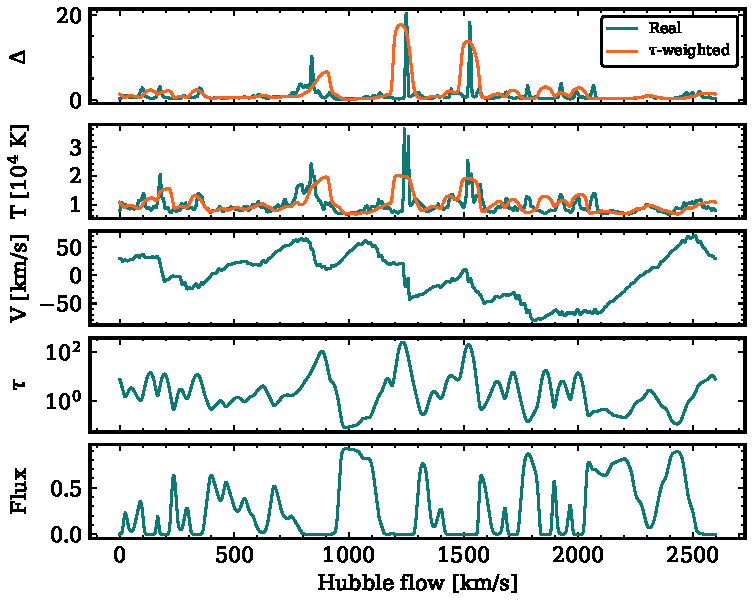
\includegraphics[width=0.95\textwidth]{img/ML/Skewer_OD_quantities.pdf}
        \caption{A 20h$^{-1}$cMpc \texttt{SHERWOOD} CDM skewer at $z=4.4$ with 2048 pixels. We show the hydrogen overdensity $\Delta$, temperature $T$ and velocity along the sightline $V$, Lyman-$\alpha$ optical depth and flux computed according to \ref{eq:lyman opacity}. We also show the optical depth-weighted overdensity and temperature, computed according to \ref{eq: OD weighted}}
        \label{fig: skewer sherwood}     
\end{figure}













\section{Statistical analysis of the effect of dark matter in the flux and density fields}\label{sec:statistics sher}


In Section \ref{sec:sherwood suite} we have presented the \texttt{SHERWOOD THERMAL} simulation suite, which include runs with the same initial seed but different thermal parameters and WDM particle masses. Naturally, challenging such parameters modify the IGM and Lyman-$\alpha$ forest properties. In this section, we explore how the density field and the Lyman-$\alpha$ forest are modified by such parameters within the \texttt{SHERWOOD} suite. In Figure \ref{fig: skewer delta flux} we show an example of this process. The figure shows the $\Delta$ overdensity and flux for 3 different WDM models in ther \texttt{SHERWOOD} suite at $z=4.4$. Note how the CDM skewers shows more fluctuations and pronounced features than the WDM models.

\begin{figure}[ht]
        \centering
            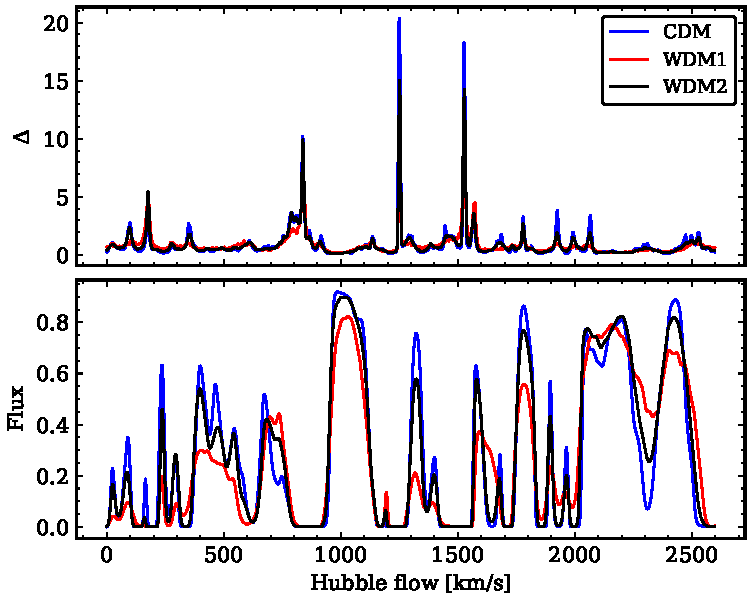
\includegraphics[width=0.99\textwidth]{img/ML/skewer_delta_flux.pdf}
            \caption{The $\Delta$ overdensity and flux for 3 different WDM models in ther \texttt{SHERWOOD} suite at $z=4.4$. Note how the CDM skewers shows more fluctuations and pronounced features than the WDM models.}
            \label{fig: skewer delta flux}
\end{figure}
To quantify this in a more robust and precise way, we leverage two summary statistics, the Probability Distribution Function (PDF) and the Power Spectrum (PS), that aggregate multiple skewers to produce quantities that only depend on the statistical proeprties of the fields, and not on the specific simulation seed for the sightline.

For a given set of sightlines, the PDF of a field is the histogram of values for such field on the array obtained concatenating the skewers. We use Numpy's \texttt{numpy.histogram} to compute it and Rice's rule to obtain the number of bins. According to this rule, for $N$ observed values, the number of bins in the histogram should be $\sim 2N^{1/3}$ \cite{Freedman1981}. For data with 2048 pixels, we use 21 bins. Since in this section we are only interested in quantifying the statistics for every model, we refer to Section \ref{sec:recovered statistics} for a discussion of the uncertainty estimation in field statistics.


\begin{figure}[ht]
        \centering
            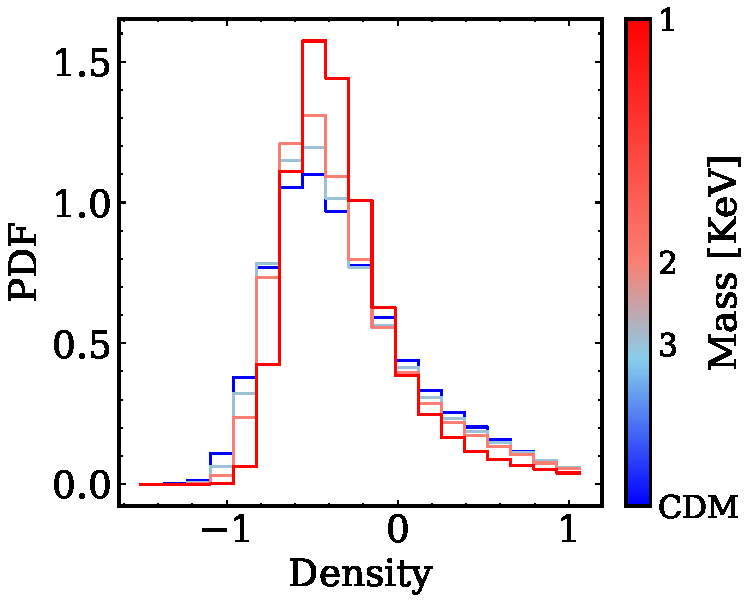
\includegraphics[width=0.8\textwidth]{img/ML/pdf_density_sherwood.pdf}
            \caption{The $\Delta_\tau$ probability distriburion function (PDF) for different WDM models in the \texttt{SHERWOOD} suite.}
            \label{fig: exact density PDF}
\end{figure}


In Figure \ref{fig: exact density PDF} we show the $\Delta_\tau$ PDF at $z=4.4$ for different WDM particle masses in the \texttt{SHERWOOD} suite. Note how low mass models tend to have a more localised distribution near the mean, which reflects the observation from Figure \ref{fig: skewer delta flux} that such models have smoother fields. In contrast, the CDM model has a greater variance, reflecting the fact that more pronounced features occur, which leads to more extreme values for the fields. 

The PDF quantifyies how often a certain value occurs, but not the correlations in the field. To study the oscilattions in the fields it is common in the literature to use the Power Spectrum (PS) \cite{McDonald_2006,Ravoux_2023}. The PS is defined in Fourier space of the relevant field, up to a normalisation factor. Here, we focus on the Lyman-$\alpha$ flux field, $F$, since it has been measured from multiple quasar samples. Since we are only interested in how $F$ oscilates, we consider the flux contrast

\begin{equation}\label{eq: flux contrast}
        \delta F=\frac{F}{\overline{F}} -1,
\end{equation}
where $\overline{F}$ is the mean value of the field. The power spectrum $P_k$ is defined as the modulus of the normalised Fourier transform of $\delta F$:

\begin{equation}\label{eq: PS def}
        P_k = \left| \mathcal{F}(\frac{1}{N} F)  \right| ^2,
\end{equation}
where $N$ is the number of pixels on a sightline (2048 for \texttt{SHERWOOD}) and $\mathcal{F}$ denotes the (Fast) Fourier Transform operator. Note that, by the Wiener-Khinchin theorem, the power spectrum is just the Fourier transform of the autocorrelation function of the $\delta F$. We compute the PS using Numpy's \texttt{numpy.fft} class. The wavenumber $k$ are binned in log space, with a spacing of $\Delta log(k)=0.1$ in the same manner as \cite{Boera_2019}. The compare the PS from the \texttt{SHERWOOD} data to real observations, we normalise the flux field to match the mean observed flux in \cite{Becker_mean_flux}. We do this by introducing a factor $a$ in the optical depth such that $F=e^{-a\tau}$ matches the mean observed flux at every redshift. Figure \ref{fig: sherwood exact PS} shows the Lyman-$\alpha$ flux power spectrum for different WDM models in the \texttt{SHERWOOD} simulation suite, compared to the observed PS by \cite{Boera_2019}. We begin by observing that WDM models have to effect of supressing structure only in the small scales (high $k$ values). At large scales, all WDM models have a similar power spectrum. Lower masses suppress the PS more than WDM models close to CDM.
In Figure \ref{fig: sherwood exact PS}, we observe a systematic bias where the Sherwood CDM power spectrum underestimates the observed power spectrum in \cite{Boera_2019}. In the original Sherwood publication \cite{Bolton_2016}, a continuous bias correction factor is applied to the flux in order to forward model the skewers, in addition to matching the observed effective optical depth. This bias correction, which has not been incorporated in this work, could be the origin of the differences observed in the figure. In the rest of the work, we will use the PDF statistic when constraining WDM, so that this PS bias will not be a concern.

\begin{figure}[ht]
        \centering
        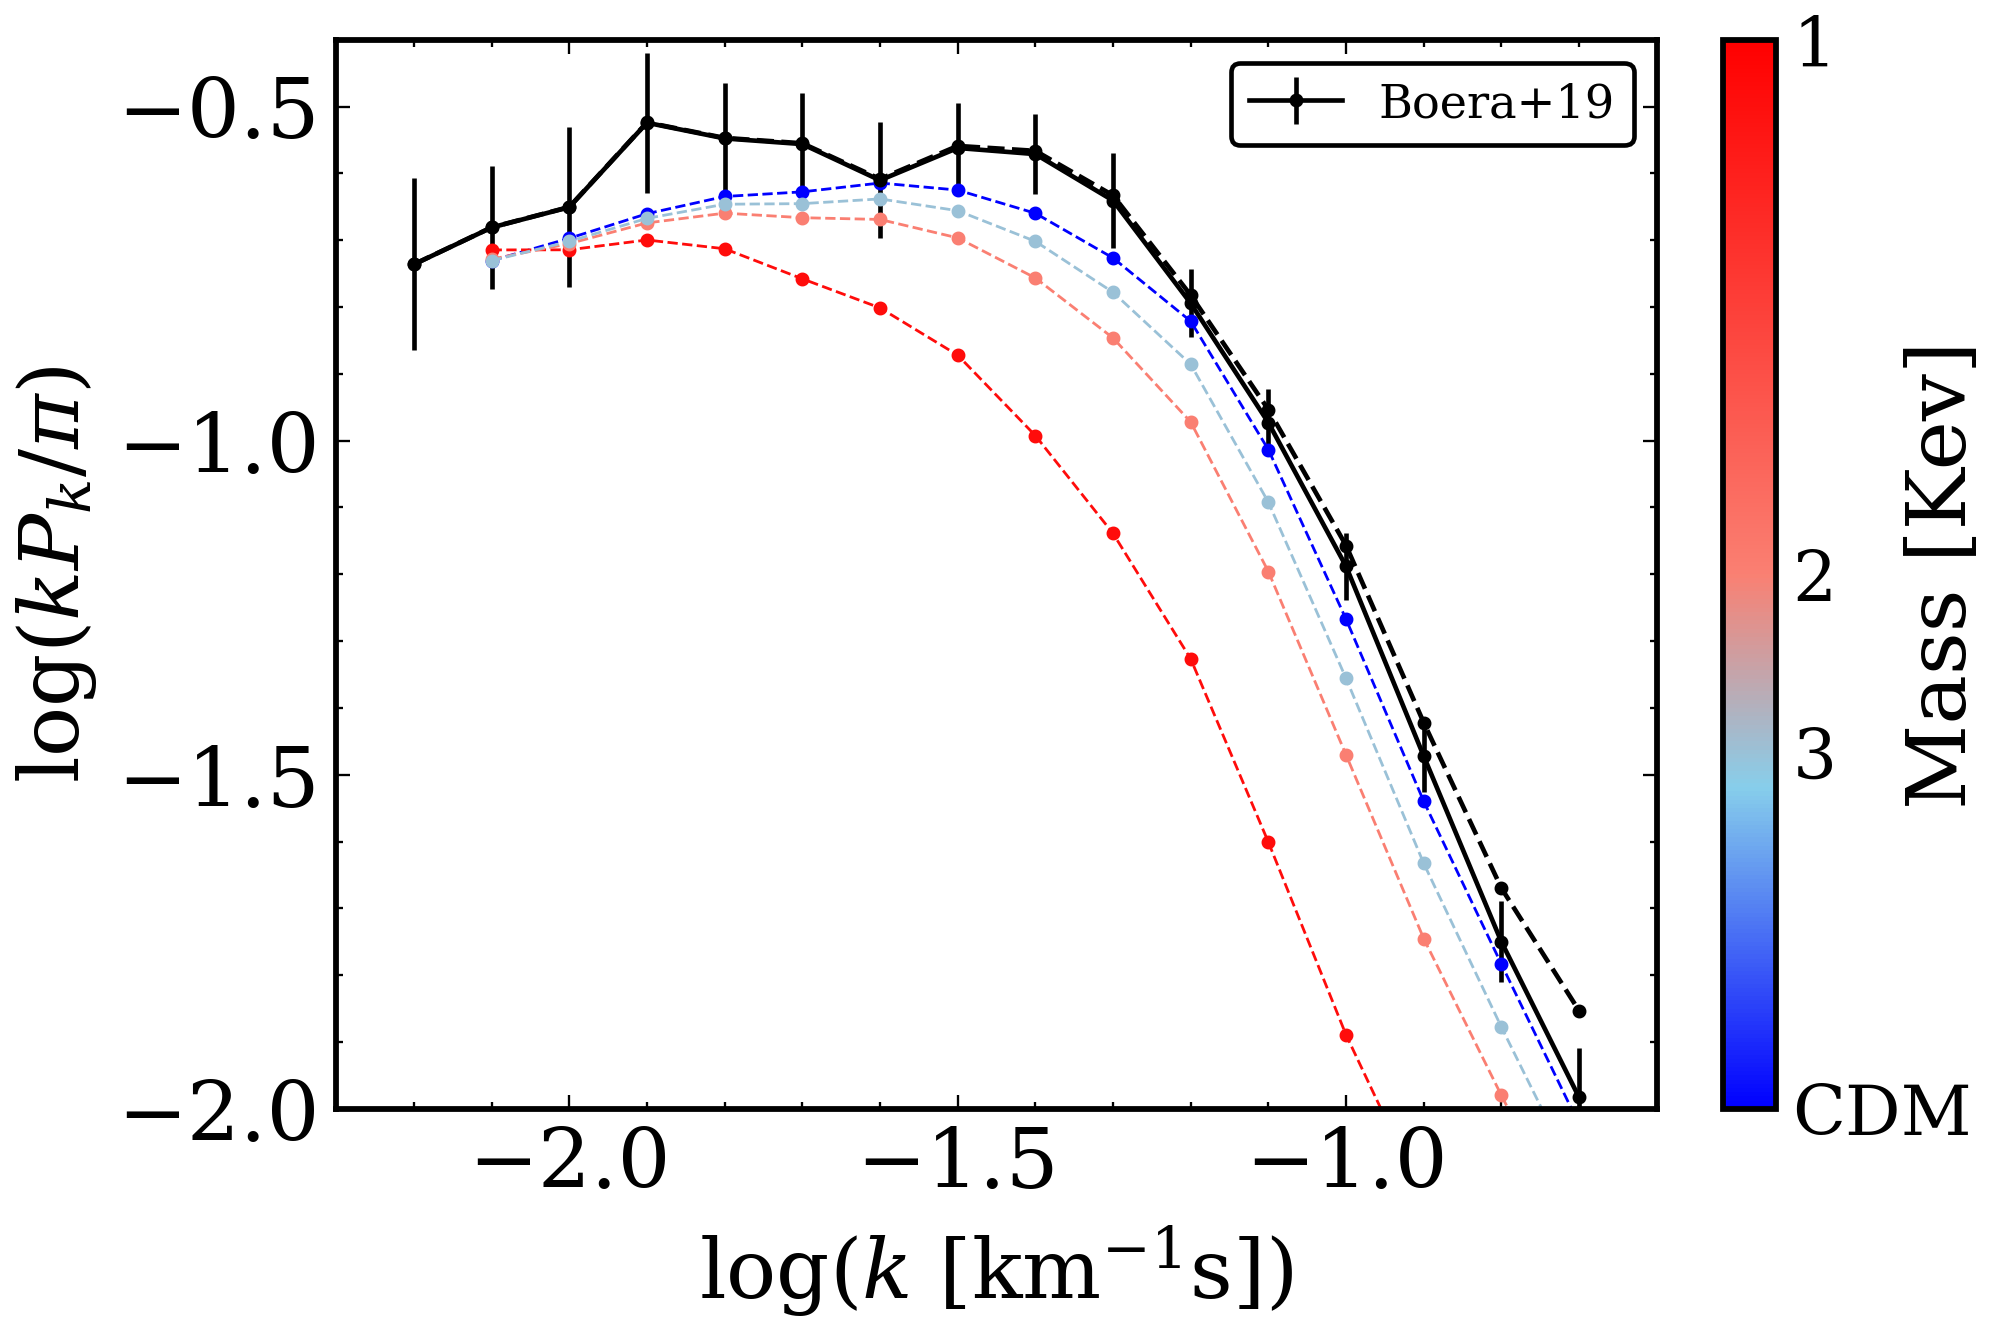
\includegraphics[width=0.99\textwidth]{img/ML/PS_sherwood.png}
        \caption{The Lyman-$\alpha$ flux power spectrum for different WDM models in the \texttt{SHERWOOD} simulation suite. For reference, we also plot the observed PS by \cite{Boera_2019}.}
        \label{fig: sherwood exact PS}     
\end{figure}


Since both the thermal state of the IGM and the WDM particle mass affect the Lyman-$\alpha$ forest, we could ask whether those two effects are degenerate. In fact, a hotter IGM means that the Voigt absoprtion profiles are wider, which smoothes out the forest at small scales, similarly to the effect how low WDM masses. If those two effects are completely degenerate, a smoother Lyman-$\alpha$ forest would not allow discriminating betweent a hotter IGM and a smalleer WDM particle mass. In Figure \ref{fig: PS thermal vs WDM} we show a comparison at $z=4.4$ of the effect of WDM models and thermal models within the \texttt{SHERWOOD THERMAL} suite on the Lyman-$\alpha$ flux power spectrum. Note that both effects are not completely degenerate. WDM models only suppress the power spectrum at small scales, while hotter models modify the power spectrum in the whole wavenumber range. As a consequence, the Lyman-$\alpha$ forest breaks the degeneracy between thermawl and WDM models.

\begin{figure}[ht]
        \centering
            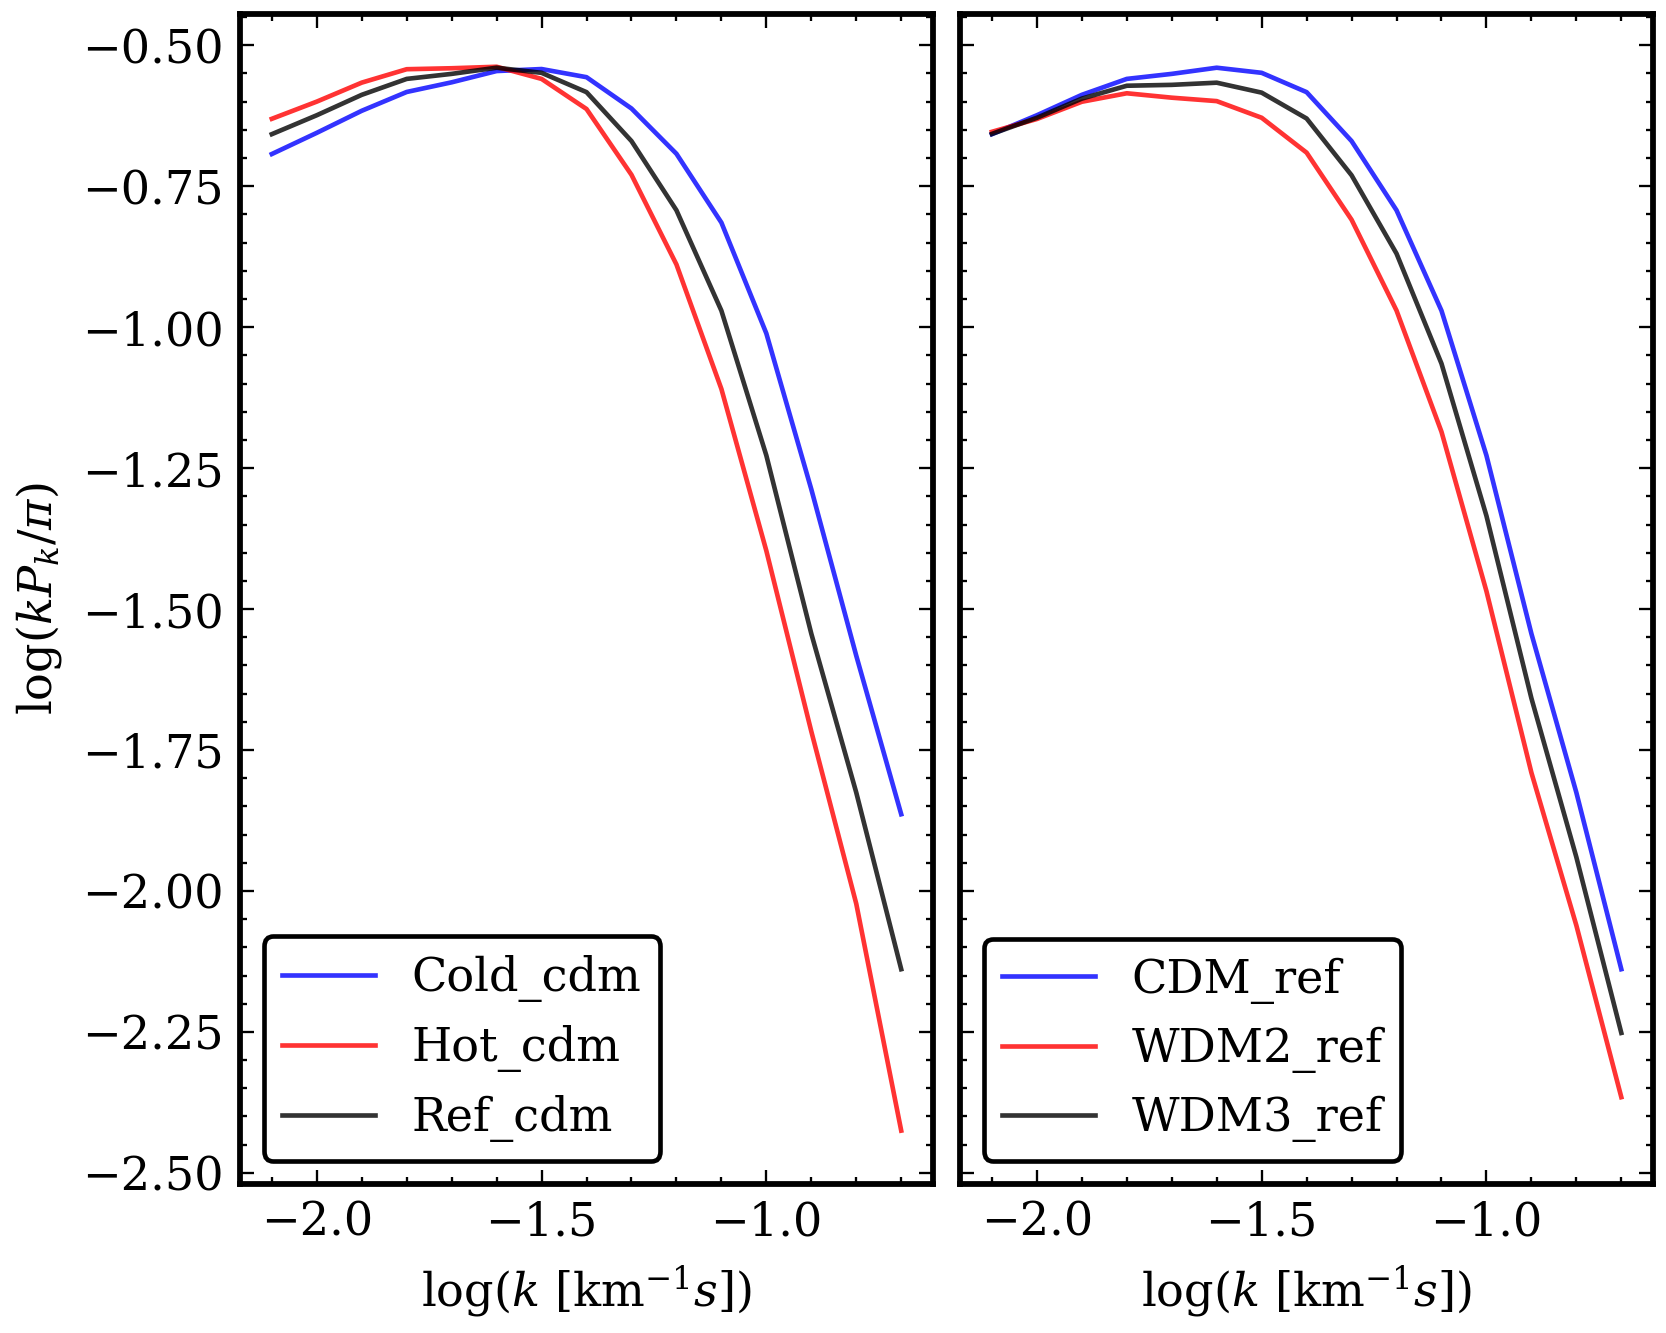
\includegraphics[width=0.8\textwidth]{img/ML/PS_thermal_vs_wdm.png}
            \caption{A comparison at $z=4.4$ of the effect of WDM models and thermal models within the \texttt{SHERWOOD} suite on the Lyman-$\alpha$ flux power spectrum. Note that both effects are not completely degenerate. WDM models only suppress the power spectrum at small scales, while hotter models modify the power spectrum in the whole wavenumber range.}
            \label{fig: PS thermal vs WDM}
\end{figure}   




